%%%%%%%%%%%%%%%%%%%%%%%%%%%%%%%%%%%%%%%%%%%%%%%%%%%%%%%%%%%%%%%%%%%%%%
% Lớp 12 | Ứng dụng đạo hàm để khảo sát hàm số | Giá trị lớn nhất và giá trị nhỏ nhất của hàm số
% Dạng 2D1?3-2: GTLN, GTNN trên khoảng
% Số câu: 23  (sinh tự động bởi tach_cau.py; từ nay thầy sửa trực tiếp file này)
%%%%%%%%%%%%%%%%%%%%%%%%%%%%%%%%%%%%%%%%%%%%%%%%%%%%%%%%%%%%%%%%%%%%%%

%%%%%%%%%%%%%%%% TRẮC NGHIỆM 4 PHƯƠNG ÁN %%%%%%%%%%%%%%%%

% nguồn: Phan1_Lop_12_Dai_so_Chuong_1
\begin{ex}%[2D1N3-2]%[ma:ccf237f9]
	Cho hàm số $y=f(x)$ có  bảng biến thiên như sau
	\begin{center}
		
\begin{tikzpicture}[scale=1,font=\footnotesize,line join=round,line cap=round,>=stealth]
			\tkzTabInit[nocadre=true,lgt=1,espcl=3,deltacl=0.5] 
				{$x$/.7,$f'(x)$/.7,$f (x)$/2} 
				{$-\infty$,$-2$,$2$,$+\infty$} 
			\tkzTabLine{,-,0,+,0,-,} 
			 \tkzTabVar{+/$+\infty$,-/$-1$,+/$3$,-/$-\infty$}
		\end{tikzpicture}
	\end{center}
	Trên khoảng  $(0;+\infty)$, giá trị lớn nhất của hàm số đã cho bằng
	\choice 
		{$-2$} 
		{\True $3$} 
		 {$-1$}
		 {$2$}
	\loigiai{ 
		Bảng biến  thiên của hàm số đã cho trên khoảng $(0\,;\,+\infty)$.
		\begin{center}
			
\begin{tikzpicture}[scale=1,font=\footnotesize,line join=round,line cap=round,>=stealth]
				 \tkzTabInit[nocadre=true,lgt=1,espcl=3,deltacl=0.5]
					{$x$/.7,$f'(x)$/.7,$f  (x)$/2}
					 {$0$,$2$,$+\infty$}
				 \tkzTabLine{,+,0,-,}
				 \tkzTabVar{-/,+/$3$,-/$-\infty$}
			\end{tikzpicture}
		\end{center}
		Dựa vào bảng  biến thiên, giá trị lớn nhất của hàm số trên khoảng $(0\,;\,+\infty)$ là $3$.
	} 
\end{ex}

% nguồn: Phan1_Lop_12_Dai_so_Chuong_1
\begin{ex}%[2D1N3-2]%[ma:f3cde87e]
	\immini{Giá trị  nhỏ nhất trên tập xác định của hàm số có đồ thị sau là
	 \choice
		{\True  $\min\limits_{\mathscr{D}} y=-1$}
		{$\min\limits_{\mathscr{D}} y=1$} 
		{$\min\limits_{\mathscr{D}} y=0$} 
		{$\min\limits_{\mathscr{D}}  y=-2$}}
		{ 
		{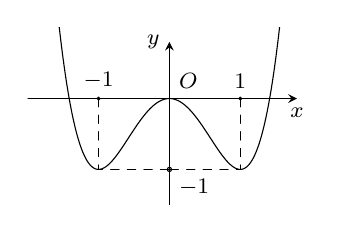
\begin{tikzpicture}[scale=0.9,>=stealth,font=\footnotesize,line join=round,line cap=round]
		\clip  (-2,-1.5) rectangle (2,1);
		\draw[->] (-2,0)--(1.8,0) node [below]{$x$}; 
		\draw[->]  (0,-1.5)--(0,0.8) node [left]{$y$};
		 \draw[samples=300,domain=-1.7:1.7]plot (\x,{(\x)^4-2*(\x)^2});
		\draw  [dashed](-1,0)|-(-1,-1)|-(0,-1);
		 \draw [dashed](1,0)|-(1,-1)|-(0,-1);
		\draw  node at (-1,0)[above]{$-1$};
		\draw node at  (1,0)[above]{$1$};
		\draw node at (0,0)[above right]{$O$}; 
		\draw  node at (0,-1)[below right]{$-1$};
		\draw  (-1,0) circle (0.2mm);
		 \draw (1,0) circle (0.2mm);
		\draw  (0,-1) circle (0.3mm);
	\end{tikzpicture}
		}} 
	\loigiai{Dựa vào đồ thị ta  có giá trị nhỏ nhất bằng $-1$.}
\end{ex}

% nguồn: Phan1_Lop_12_Dai_so_Chuong_1
\begin{ex}%[2D1H3-2]%[ma:15277bba]
	Tìm giá trị lớn nhất  $M$ của hàm số $y=-2\sqrt{4-x}$.
	\choice 
		{$M=-4$} 
		 {$M=-2$}
		{$M=1$} 
		{\True  $M=0$}
	\loigiai{ 
		 Điều kiện: $4-x\leq 0 \Leftrightarrow x\leq 4$. \\
		Ta có $y=-2\sqrt{4-x}\leq 0$, $\forall  x\leq 4$. Đẳng thức xảy ra khi $x=4$.\\
	 Do đó $M=\max\limits_{(-\infty;4]}y=0$.}
\end{ex}

% nguồn: Phan1_Lop_12_Dai_so_Chuong_1
\begin{ex}%[2D1H3-2]%[ma:8a9d20c2]
	Giá trị lớn nhất  của hàm số $f(x)=x(1-x^2)$ trên khoảng $(0;1)$ là
	\choice 
		 {$\dfrac{1}{9}$}
		{$\dfrac{1}{\sqrt{3}}$} 
		 {$0$}
		{\True  $\dfrac{2\sqrt{3}}{9}$}
	 \loigiai{
		$f'(x)=0\Leftrightarrow x=\pm \dfrac{1}{\sqrt{3}}  \in (0;1)$.\\
		Hàm số $y=f(x)$ liên tục trên $(0;1)$,  đồng thời
		$\lim\limits_{x\to  0^+}f(x)=0$, $\lim\limits_{x\to 1^-}f(x)=0$.\\
		Mặt khác $f\left(\dfrac{1}{\sqrt{3}}\right)=\dfrac{2\sqrt{3}}{9}$;  $f\left(-\dfrac{1}{\sqrt{3}}\right)=-\dfrac{2\sqrt{3}}{9}$.\\
		Nên $\max\limits_{(0;1)}  f(x)=\dfrac{2\sqrt{3}}{9}$.
	} 
\end{ex}

% nguồn: Phan1_Lop_12_Dai_so_Chuong_1
\begin{ex}%[2D1H3-2]%[ma:36488f8f]
	 Tìm giá trị lớn nhất $M$ của hàm số $y=\dfrac{x+1}{\sqrt{x^2+1}}$ trên khoảng $\left( {-\infty;+\infty} \right)$.
	 \choice
		 {$M=2\sqrt{2}$}
		{$M=1$} 
		 {\True $M=\sqrt{2}$}
		{$M=2$} 
	 \loigiai{
		Ta có $y'=0 \Leftrightarrow \dfrac{1-x}{\left( {x^2+1} \right)\sqrt{x^2+1}}=0 \Leftrightarrow x=1$. 
		\\Bảng  biến thiên
		\begin{center}
			
\begin{tikzpicture}[scale=0.8]
				\tkzTabInit 
					 [lgt=3,espcl=3]
					 {$x$/1.2,$y'$/1,$y$/2.5}
					 {$-\infty$,$1$,$+\infty$}
				 \tkzTabLine{,+,0,-,}
				\tkzTabVar{-/ $-1$,+/ $\sqrt{2}$,-/ $1$} 
			\end{tikzpicture}
		\end{center}
	Dựa vào bảng biến thiên ta thấy giá  trị lớn nhất của hàm số là $M=\sqrt{2}$.}
\end{ex}

% nguồn: Phan1_Lop_12_Dai_so_Chuong_1
\begin{ex}%[2D1H3-2]%[ma:2a6d8edc]
	Cho hàm số $y=x^3-\dfrac{3}{2}  x^2+1$. Gọi $M$ là giá trị lớn nhất của hàm số trên khoảng $\left(-25;\dfrac{11}{10} \right)$. Tìm giá trị của $M$.
	 \choice
		{\True  $M=1$}
		{$M=\dfrac{1}{2}$} 
		 {$M=0$}
		{$\dfrac{129}{250}$} 
	\loigiai{ 
		Tập xác  định $\mathscr D=\mathbb{R}$.\\
		 Ta có $y'=3x^2-3x$.\\
		Cho $y'=0\Leftrightarrow  \hoac{&x=0 \\ &x=1.}$\\
		Bảng biến thiên 
		\begin{center}
			
\begin{tikzpicture}
				\tkzTabInit 
					 [lgt=1.5,espcl=2]
					 {$x$/1.2,$f’(x)$/1,$f (x)$/2}
					 {$-25$,$0$,$1$,$\dfrac{11}{10}$}
				 \tkzTabLine{,+,0,-,0,+,}
				\tkzTabVar{-/$-\tfrac{33\,123}{2} $,+/ $1$,-/$f  (0)$,+/$\tfrac{129}{250}$}
			\end{tikzpicture}
		\end{center}
		Vậy $M=f(0)=1$. 
	} 
\end{ex}

% nguồn: Phan1_Lop_12_Dai_so_Chuong_1
\begin{ex}%[2D1H3-2]%[ma:c2ffffb1]
	 Giá trị lớn nhất của hàm số $y=\sqrt{x+2}-x$ là
	\choice 
		{$-\dfrac{5}{4}$} 
		{$\sqrt{3}-1$} 
		 {\True $\dfrac{9}{4}$}
		{$2$} 
	 \loigiai{
		Tập xác định $\mathscr{D}=[-2;+\infty)$.  \\
		Ta có  $y' =\dfrac{1}{2\sqrt{x+2}}-1\Rightarrow y'=0\Leftrightarrow x=-\dfrac{7}{4}$.\\
		 Bảng biến thiên
		\begin{center}
			
\begin{tikzpicture}[scale=1,line join=round,line cap=round]
				\tkzTabInit[nocadre=false,lgt=1,espcl=2.5] 
					{$x$ /1,$y'$ /0.8,$y$  /2}
					 {$-2$,$-\dfrac{7}{4}$,$+\infty$}
				 \tkzTabLine{,+,$0$,-,}
				 \tkzTabVar{-/$2$,+/$\dfrac{9}{4}$,-/$-\infty$}
			\end{tikzpicture}
		\end{center}
		Từ bảng biến thiên ta có $\max\limits_{\mathscr{D}}  y=\dfrac{9}{4}$.
	 }
\end{ex}

% nguồn: Phan1_Lop_12_Dai_so_Chuong_1
\begin{ex}%[2D1H3-2]%[ma:42404e3a]
	Giá  trị lớn nhất của hàm số $y = 2x + \dfrac{1}{x}$ khi $x < 0$ là
	 \choice
		{$2\sqrt{2}$} 
		 {\True $-2\sqrt{2}$}
		{Không  tồn tại}
		 {$4$}
	 \loigiai{
		 Với $x < 0$, ta có $y'=2-\dfrac{1}{x^2}=\dfrac{2x^2-1}{x^2}$.\\
		$y'=0\Leftrightarrow \hoac{&x=\dfrac{\sqrt{2}}{2}\  \text{ (loại)}\\&x=-\dfrac{\sqrt{2}}{2}\ \text{ (nhận)}.}$\\
		Bảng biến thiên 
		\begin{center}
			
\begin{tikzpicture}
				\tkzTabInit[espcl=2.5,lgt=1.5] 
					{$x$/1,$y'$/0.7,$y$/2.1} 
					{$-\infty$,$-\dfrac{\sqrt{2}}{2}$,$0$} 
				\tkzTabLine{,+,0,-} 
				 \tkzTabVar{-/$-\infty$,+/$-2\sqrt{2}$,-/$-\infty$}
			\end{tikzpicture}
		\end{center}
		Vậy giá trị lớn nhất của hàm  số $y = 2x + \dfrac{1}{x}$ khi $x < 0$ là $-2\sqrt{2}$.
	 }
\end{ex}

% nguồn: Phan1_Lop_12_Dai_so_Chuong_1
\begin{ex}%[2D1H3-2]%[ma:b0407970]
	Giá trị lớn nhất của hàm số $y=-x^3+3 x+1$ trên khoảng  $(0;+\infty)$ bằng
	\choice 
		 {$1$}
		{\True $3$} 
		 {$-1$}
		{$5$} 
	\loigiai{Ta có $y'=-3 x^2+3$, $y'=0 \Leftrightarrow  \hoac{&x=1\in(0;+\infty) \\&x=-1 \notin(0;+\infty)}$.\\
		 Bảng biến thiên
		\begin{center}
			
\begin{tikzpicture}
				\tkzTabInit[nocadre=false,lgt=0.7,espcl=2.5,deltacl=0.5] 
					{$x$ /0.7,$y'$ /0.7,$y$ /2} 
					{$0$,$1$,$+\infty$} 
				\tkzTabLine{,+,$0$,-,} 
				\tkzTabVar{-/$1$,+/$3$,-/$-\infty$} 
			\end{tikzpicture}
		\end{center}
	Từ bảng biến thiên ta thấy giá trị lớn nhất  của hàm số $y=-x^3+3 x+1$ trên khoảng $(0;+\infty)$ bằng 3.}
\end{ex}

% nguồn: Phan1_Lop_12_Dai_so_Chuong_1
\begin{ex}%[2D1V3-2]%[ma:c224f84f]
	Cho hàm số $y=f(x)$ có đạo hàm cấp  hai trên $\mathbb{R}$. Biết $f'(0)=3$, $f'(2)=-2$ và bảng xét dấu của $f''(x)$ như sau
	\begin{center}
		
\begin{tikzpicture}
			 \tkzTabInit[nocadre=false,lgt=1.2,espcl=2.5]
				{$x$ /0.6,$f''(x)$ /0.6} 
				{$-\infty$,$0$,$2$,$+\infty$} 
			 \tkzTabLine{,+,$0$,-,$0$,+,}
		\end{tikzpicture}
	\end{center}
	Hàm số $y=f(x+3)+2x$ đạt giá trị nhỏ nhất tại điểm $x_0$ thuộc khoảng  nào sau đây?
	\choice 
		 {$(3;+\infty)$}
		{\True $(-\infty;-3)$} 
		 {$(0;3)$}
		 {$(-2;0)$}
	\loigiai{ 
		Từ bảng xét dấu của $f''(x)$ ta có bảng biến thiên của  $f'(x)$ như sau
		\begin{center}
			
\begin{tikzpicture}
				 \tkzTabInit[nocadre=false,lgt=2,espcl=2.5]
					{$x$  /0.6,$f''(x)$ /0.6,$f'(x)$ /2,$f'(x)+2$/2}
					 {$-\infty$,$0$,$2$,$+\infty$}
				\tkzTabLine{,+,$0$,-,$0$,+,} 
				\tkzTabVar{-/$-\infty$,+/$3$,-/$-2$,+/$+\infty$} 
				\tkzTabVar{-/$-\infty$,+/$5$,-/$0$,+/$+\infty$} 
			\end{tikzpicture}
		\end{center}
		Từ BBT, ta thấy $f'(x)+2=0\Leftrightarrow  \hoac{&x=2\\&x=a<0.}$\\
		Ta có BBT của  $y=f(x)+2x$ như sau
		\begin{center}
			
\begin{tikzpicture}
				\tkzTabInit[nocadre=false,lgt=2,espcl=2.5] 
					{$x$ /0.6,$f'(x)+2$  /0.6,$f (x)+2x$ /2}
					{$-\infty$,$a$,$2$,$+\infty$} 
				 \tkzTabLine{,-,$0$,+,$0$,+,}
				\tkzTabVar{+/$+\infty$,-/$f  (a)+2a$,R,+/$+\infty$}
			\end{tikzpicture}
		\end{center}
		Từ BBT, ta thấy hàm số $y=f(x)+2x$ đạt GTNN tại $x=a, (a<0)$.\\ 
		Vậy hàm số $y=f(x+3)+2x$ đạt GTNN  tại $x=a-3$.
	 }
\end{ex}


%%%%%%%%%%%%%%%% ĐÚNG/SAI %%%%%%%%%%%%%%%%

% nguồn: Phan1_Lop_12_Dai_so_Chuong_1
\begin{ex}%[2D1H3-2]%[ma:7c8e3c80]
	Cho hàm số $f(x)=-x^3+3 x+10$. 
	\choiceTF 
		 {$f'(x)=-x^2+1$}
		{\True $f'(x)>0 \Leftrightarrow x \in(-1; 1)$, $f'(x)<0 \Leftrightarrow  x \in(-\infty;-1) \cup(1;+\infty)$}
		{\True $f(1)=12, f(-1)=8$} 
		{Hàm số đạt giá trị nhỏ nhất bằng $8$ tại  $x_1=-1$, đạt giá trị lớn nhất bẳng 12 tại $x_2=1$}
	 \loigiai{
		\begin{itemchoice}
			\itemch Sai. Vì  $f'(x)=-3x^2+3$.
			\itemch Đúng. 
			 \itemch Đúng.
			\itemch Sai. Vì hàm số bậc  ba $f(x)=-x^3+3 x+10$ không có giá trị nhỏ nhất và không có giá trị lớn nhất.
		\end{itemchoice}
	 }
\end{ex}

% nguồn: Phan1_Lop_12_Dai_so_Chuong_1
\begin{ex}%[2D1H3-2]%[ma:0b6d4e57]
	Cho hàm số  $y=x+\dfrac{4}{x},\, x\in \left(0;+\infty \right)$.
	 \choiceTF
		{\True  Hàm số đạt giá trị nhỏ nhất tại $x=2$ và không có giá trị lớn nhất trên $\left(0;+\infty \right)$}
		{Hàm số có giá trị lớn nhất và giá  trị nhỏ nhất trên $\left(0;+\infty \right)$}
		{Hàm số đạt giá  trị lớn nhất tại $x=1$ và không có giá trị nhỏ nhất trên khoảng $\left(0;+\infty \right)$}
		{Hàm số không có giá trị  nhỏ nhất và không có giá trị lớn nhất trên $\left(0;+\infty \right)$}
	 \loigiai{
		Ta có $y=x+\dfrac{4}{x}  \Rightarrow y'=1-\dfrac{4}{x^2}=\dfrac{x^2-4}{x^2}$.\\
		 Cho $y'=0\Leftrightarrow \dfrac{x^2-4}{x^2}=0\Leftrightarrow x=\pm 2$.\\
		Bảng biến thiên của  hàm số $y=x+\dfrac{4}{x}, x\in \left(0;+\infty \right)$.
		\begin{center}
			
\begin{tikzpicture}
				 \tkzTabInit
					 [lgt=1.5,espcl=2]
					 {$x$/1.2,$y'$/1,$y$/2}
					{$0$,$2$,$+\infty$} 
				 \tkzTabLine{,-,0,+,}
				\tkzTabVar{+/  $+\infty $,-/ $0 $,+/ $+\infty$}
			\end{tikzpicture}
		\end{center}
		\noindent 
		Căn cứ vào bảng biến thiên ta có hàm số đạt giá trị nhỏ nhất tại $x=2$  và không có giá trị lớn nhất trên $\left(0;+\infty \right)$.
	} 
\end{ex}

% nguồn: Phan1_Lop_12_Dai_so_Chuong_1
\begin{ex}%[2D1H3-2]%[ma:b8b838ac]
	\immini{Cho hàm số $y=f(x)$ liên tục trên $\mathbb{R}$ và có đồ thị  như hình bên.
	 \choiceTF
		{\True Hàm số nghịch biến trên khoảng  $(0;1)$}
		{Hàm số đồng biến trên khoảng $(-1;2)$} 
		{\True Hàm số có  ba điểm cực trị}
		{Hàm số có giá trị lớn  nhất bằng $2$}
		}{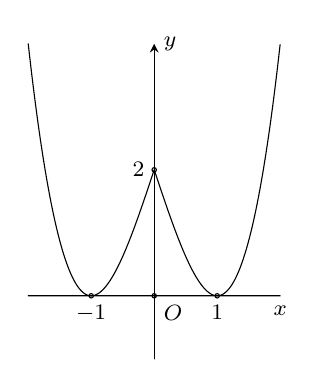
\begin{tikzpicture}[scale=0.8,font=\footnotesize,line join=round,line join=round,line cap = round,>=stealth]
		\draw[->] (-2,0)--(0,0) node[below right]{$O$} circle (1pt)--(2,0)  node[below]{$x$};
		 \draw[->] (0,-1) --(0,4) node[right]{$y$};
		\foreach  \x in {-1,1}{
			\draw  (\x,0) node[below]{$\x$} circle (1pt);}
		\foreach \y in {2}{ 
			\draw (0,\y) node[left]{$\y$} circle (1pt);} 
		 \draw [domain=0:2,samples=100]
			plot  (\x,{(\x)^3-3*(\x)+2});
		 \draw [domain=-2:0,samples=100]
			plot (\x,{-(\x)^3+3*(\x)+2}); 
	\end{tikzpicture}
		 }
	 \loigiai{
		Dựa vào đồ thị hàm số,  ta thấy
		\begin{itemchoice}
			\itemch Hàm số nghịch biến trên khoảng  $(0;1)$ là khẳng định đúng.
			\itemch Hàm số đồng biến trên khoảng $(-1;2)$ là khẳng định sai,  vì trên khoảng $(0;1)$ hàm số nghịch biến.
			\itemch Hàm số  có ba điểm cực trị là khẳng định đúng, hàm số có $3$ điểm cực trị tại $x=-1$, $x=0$, $x=1$.
			\itemch Hàm số có giá trị lớn nhất bằng  $2$ là khẳng định sai, hàm số có giá trị cực đại bằng $2$, không tồn tại giá trị lớn nhất.
		\end{itemchoice}
	} 
\end{ex}

% nguồn: Phan1_Lop_12_Dai_so_Chuong_1
\begin{ex}%[2D1H3-2]%[ma:88a61226]
	Cho hàm số $y=f(x)$ xác định và liên tục trên $\left(-4;4\right)$ và có bảng biến  thiên như sau:
	\begin{center}
		
\begin{tikzpicture}
			\tkzTabInit 
				[lgt=1.5,espcl=3] 
				 {$x$/1.2,$f’(x)$/1,$f (x)$/2}
				 {$-4$,$-2$,$0$,$4$}
			\tkzTabLine{,+,0,-,0,+,} 
			\tkzTabVar{-/ $-10$,+/  $0 $,-/ $-4 $,+/ $10$}
		\end{tikzpicture}
	\end{center}
	 \choiceTF
		{${\mathop{\min}\limits_{\left(-4;4\right)}} y=-4$  và ${\mathop{\max}\limits_{\left(-4;4\right)}} y=10$}
		{${\mathop{\max}\limits_{\left(-4;4\right)}}  y=10$ và ${\mathop{\min}\limits_{\left(-4;4\right)}} y=-10$}
		 {${\mathop{\max}\limits_{\left(-4;4\right)}} y=0$ và ${\mathop{\min}\limits_{\left(-4;4\right)}} y=-4$}
		{\True Hàm số không có giá trị lớn nhất và nhỏ nhất trên  $\left(-4;4\right)$}
	 \loigiai{
	Dựa vào bảng biến thiên, ta thấy hàm số không có giá trị lớn nhất và nhỏ nhất  trên $\left(-4;4\right)$.}
\end{ex}


%%%%%%%%%%%%%%%% TRẢ LỜI NGẮN %%%%%%%%%%%%%%%%

% nguồn: Phan2_Lop_12_Dai_so_Chuong_1
\begin{bt}%[2D1H3-2]%[ma:259b3a31]
	Cho hàm số $y=\dfrac{mx-m^2-2}{x-1}$ ($m$  là tham số thực) thoả mãn $\max\limits_{[-2;0]}y=3$. Có bao nhiêu giá trị dương của $m$ thoả mãn điều kiện bài toán?
	\shortans{1} 
	\loigiai{Ta có  $y'=\dfrac{m^2-m+2}{(x-1)^2}>0$ với $\forall x\in[-2;0]$.\\
		 Suy ra hàm số $y=\dfrac{mx-m^2-2}{x-1}$ đồng biến trên $[-2;0]$, suy ra $\max\limits_{[-2;0]}y=y(0)=m^2+2$.\\
		 Theo đề bài suy ra $m^2+2=3$, suy ra $m=\pm1$ mà $m>0$ nên ta nhận giá trị $m=1$.\\
	Vậy có $1$ giá trị dương của $m$  thoả mãn điều kiện bài toán.}
\end{bt}

% nguồn: Phan2_Lop_12_Dai_so_Chuong_1
\begin{bt}%[NBV2526]%[2D1H3-2]%[ma:2dbfcdf6]
	Vận tốc của một tàu con thoi từ lúc cất cánh tại thời điểm $t=0$ (s) cho đến thời điểm $t=126$ (s) được cho bởi công thức $v(t) = 0{,}001302t^3 - 0{,}09029t^2 + 83$ (vận tốc được tính bằng đơn vị $\mathrm{ft/s}$). Hỏi tại thời điểm tàu con thoi đạt gia tốc nhỏ nhất thì vận tốc tàu con thoi gần bằng bao nhiêu? (Kết quả làm tròn đến hàng phần  mười).
	\shortans{20,8} 
	 \loigiai{
		Ta có: gia tốc $a(t) = v'(t) = 0{,}003906t^2 - 0{,}18058t$.\\ 
		Ta có bảng biến thiên hàm  $a(t) = 0{,}003906t^2 - 0{,}18058t$.
		\begin{center}
			
\begin{tikzpicture}[>=stealth,scale=1]
				\tkzTabInit[lgt=1.5,espcl=3.5] 
					{$t$ /.7,$a'(t)$ /.7,$a (t)$  /1.8}
					{$-\infty$,$23{,}1157$,$+\infty$} 
				 \tkzTabLine{,-,$0$,+,}
				 \tkzTabVar{+/,-/$2{,}087$,+/}
			\end{tikzpicture}
		\end{center}
		Thời điểm tàu con thoi đạt gia  tốc nhỏ nhất là $t \approx 23{,}1157$.\\
		Vậy  $v(23{,}1157) = 0{,}001302\cdot (23{,}1157)^3 - 0{,}09029\cdot (23{,}1157)^2 + 83 \approx 20{,}8~\mathrm{ft/s}.$
	 }
\end{bt}

% nguồn: Phan2_Lop_12_Dai_so_Chuong_1
\begin{bt}%[2D1H3-2]%[ma:219e54e6]
	Cho hàm số $f(x)=4 x^{3}-9 x^{2}-30 x$. Với các số nguyên $a, b$  mà $a<b$ thì giá trị nhỏ nhất của $f(b)-f(a)$ bằng bao nhiêu?\shortans{-81}
	 \loigiai{
		Ta  có $f^{\prime}(x)=12 x^{2}-18 x-30=0 \Leftrightarrow\hoac{&x=-1 \\& x=\dfrac{5}{2}}.$\\ Bảng biến thiên
		\begin{center}
			
\begin{tikzpicture}
				 \tkzTabInit
					[lgt=1.5,espcl=2.5] 
					{$x$/1.2,$f’(x)$/1,$f (x)$/2} 
					{$-\infty$,$-1$,$\dfrac{5}{2}$,$+\infty$} 
				 \tkzTabLine{,+,0,-,0,+,}
				 \tkzTabVar{-/ $-\infty $,+/ $ 17 $,-/ $ -\dfrac{275}{4}$,+/ $+\infty$}
			\end{tikzpicture}
		\end{center}
		\noindent 
		Ta có $f(x) =0  \Leftrightarrow \hoac{&x \approx -1{,8}\\&x=0 \\&x\approx 4{,}1.}$\\
		Với  các số nguyên $a,$ $ b$ mà $a<b$, để $f(b)-f(a)$ đạt giá trị nhỏ nhất thì $\heva{&f(b)<0 \\& f(a)>0.}$\\
		Suy ra  $ f(b)=f(2)=-64$; $f(a)=f(-1)=17$.\\
		Vậy giá trị nhỏ nhất  của $f(b)-f(a)$ bằng $-81$.
	 }
\end{bt}

% nguồn: Phan2_Lop_12_Dai_so_Chuong_1
\begin{bt}%[2D1H3-2]%[ma:1b99f6dd]
	Giá trị nhỏ nhất của  hàm số $P=\log^2 x+\dfrac{1}{\log^2 x+2}$ bằng bao nhiêu?
	\shortans{0,5} 
	\loigiai{ 
		Đặt $t=\log^2 x+2 \geq 2, \forall  x >0$. Suy ra $f(t)=t+\dfrac{1}{t}-2$ với $t\geq 2$.\\
		Ta có $f'(t)=1-\dfrac{1}{t^2}=\dfrac{t^2-1}{t^2} > 0, \forall  t \geq 2$.\\
		Suy ra hàm số $f(t)$ đồng biến  trên $[2;+\infty)$.\\
		Vậy $\min  P= f(2)=0{,}5$.
	 }
\end{bt}

% nguồn: Phan2_Lop_12_Dai_so_Chuong_1
\begin{bt}%[2D1V3-2]%[ma:ab89fc33]
	Cho hàm số $y=\dfrac{3-m \sqrt{3} \cdot \cos x}{\sin x+2}$. Có bao nhiêu giá trị nguyên của tham  số $m$ thuộc đoạn $[-2025; 2025]$ để giá trị lớn nhất của hàm số lớn hơn $4$?
	\shortans{4048} 
	 \loigiai{Hàm số đã cho xác định $\forall x \in \mathbb{R}$ do $\sin x+2>0, \forall x \in \mathbb{R}$.\\
		Ta có \begin{eqnarray*}
		& &y=\dfrac{3-m \sqrt{3} \cdot  \cos x}{\sin x+2} \\
		&\Leftrightarrow& y \sin x+2 y=3-m \sqrt{3} \cdot \cos  x\\
		&\Leftrightarrow& y \sin  x+m \sqrt{3} \cos x=3-2y\\
		&\Leftrightarrow& \sqrt{y^{2}+(m  \sqrt{3})^{2}}\left(\dfrac{y}{\sqrt{y^{2}+(m \sqrt{3})^{2}}}\sin x + \dfrac{m\sqrt{3}}{\sqrt{y^{2}+(m \sqrt{3})^{2}}}\sin x \right)=3-2y\\
		 &\Leftrightarrow& \sqrt{y^{2}+(m \sqrt{3})^{2}}\sin(\alpha +x) = 3-2y
	\end{eqnarray*}
	Phương trình có nghiệm khi  và chỉ khi
	\begin{eqnarray*}
		&&y^{2}+(m \sqrt{3})^{2}  \geq(3-2 y)^{2}\\
		&\Leftrightarrow& y^{2}-4 y+3-m^{2} \leq  0\\
		&\Leftrightarrow&(y-2)^{2} \leq  m^{2}+1\\
		&\Leftrightarrow&|y-2| \leq  \sqrt{m^{2}+1}\\
		&\Leftrightarrow&-\sqrt{m^{2}+1} \leq y-2 \leq \sqrt{m^{2}+1}\\ 
		&\Leftrightarrow& 2-\sqrt{m^{2}+1} \leq y \leq 2+\sqrt{m^{2}+1}. 
	\end{eqnarray*}
	Suy ra giá trị lớn nhất của hàm số đã cho bằng $2+\sqrt{m^{2}+1}$.\\ 
	Ta có $2+\sqrt{m^{2}+1}>4  \Leftrightarrow \sqrt{m^{2}+1}>2 \Leftrightarrow m^{2}-3>0 \Leftrightarrow\hoac{&m<-\sqrt{3} \\ &m>\sqrt{3}.}$\\
	Vì $m$ là  số nguyên thuộc đoạn $[-2022; 2022]$
	nên $m \in\{-2025;-2021; \ldots;-3;-2; 2; 3;  4; \ldots; 2025\}$.\\
Vậy có $4048$  giá trị $m$ thỏa mãn yêu cầu bài toán.}
\end{bt}

% nguồn: Phan2_Lop_12_Dai_so_Chuong_1
\begin{bt}%[2D1V3-2]%[ma:b1bb3598]
	\immini{Người ta muốn làm một chiếc hộp kim loại hình hộp chữ nhật có thể tích $72$\,cm$^3$ và đáy có chiều dài gấp đôi chiều rộng như hình vẽ. Tính diện tích toàn phần nhỏ nhất  đạt được của chiếc hộp (kết quả làm tròn đến hàng đơn vị của cm$^2$).}{
	\begin{tikzpicture}[line join=round,line cap=round,>=stealth]
		\coordinate (A) at  (0,0);
		\coordinate  (B) at (-1.3,-1.5);
		\coordinate  (D) at (3.5,0);
		\coordinate (C) at ($(B)+(D)-(A)$); 
		\coordinate (A') at  ($(A)+(0,2.5)$);
		\coordinate (B')  at ($(B)+(0,2.5)$);
		\coordinate (C') at ($(C)+(0,2.5)$); 
		\coordinate (D') at ($(D)+(0,2.5)$); 
		 \draw (B')--(B)--(C)--(D)--(D')--(A')--(B')--(C')--(D')
			(C')--(C); 
		\draw[dashed] (B)--(A)--(D) 
			 (A)--(A');
		\node  at (0.8,-1.5) [below]{$2x$\,cm};
		\node at (3.4,-0.5) [below]{$x$\,cm}; 
		\node at  (3.5,1.25) [right]{$h$\,cm};
	\end{tikzpicture}
	 }
	\shortans{108} 
	 \loigiai{
		Ta có $x\cdot 2x\cdot h=72 \Rightarrow  h=\dfrac{36}{x^2}$.\\
		Diện tích toàn phần của chiếc  hộp là
		 $$S(x)=2(x\cdot 2x+xh+2xh)=2\left(2x^2+3xh\right)=4x^2+\dfrac{216}{x},\, x>0.$$
		 Ta có $S'(x)=8x-\dfrac{216}{x^2}$ suy ra $S'(x)=0 \Leftrightarrow x^3=27 \Leftrightarrow x=3$.\\
		Bảng biến thiên 
		\begin{center}
			
\begin{tikzpicture}
				\tkzTab[nocadre,lgt=2,espcl=2.5]{$x$/1,$S’(x)$/1,$S (x)$/2} 
					{$0$,$3$,$+\infty$} 
					{d,-,0,+,} 
					{+D+/ $ $  / $+\infty$,-/ $108$,+/ $+\infty$}
			\end{tikzpicture}
		\end{center}
		Vậy diện tích toàn phần nhỏ nhất của chiếc hộp  là $108$\,cm$^2$.
	} 
\end{bt}

% nguồn: Phan2_Lop_12_Dai_so_Chuong_1
\begin{bt}%[2D1V3-2]%[ma:6f9eb05f]
	\immini{Một xưởng thủ công mỹ nghệ sản xuất loại chụp đèn trang trí dạng hình chóp cụt tứ giác đều (như hình bên). Gọi $x$ là độ dài cạnh đáy lớn (đơn vị: dm). Tính toán cho thấy tổng chi phí vật liệu (tính bằng nghìn đồng) cho một chụp đèn là $C(x)=x^2+108$ (nghìn đồng). Thời gian sản xuất cho một chụp đèn được xác định là $T(x)=x+6$ (giờ). Xưởng muốn xác định kích thước $x$ để chi phí vật liệu trung bình trên  một giờ sản xuất là thấp nhất, nhằm tối ưu hóa hiệu quả sử dụng thời gian và vật liệu. Hãy tìm giá trị của $x$.}
	{\begin{tikzpicture}[>=stealth,line join=round,line
			 cap=round,font=\footnotesize,scale=0.7]
		 \path (0,0) coordinate (D)
			 (6,0) coordinate (C)
			(-3,-2) coordinate (A) 
			 ($(C)-(D)+(A)$) coordinate (B)
			($(A)!1/2!(C)$)  coordinate (O)
			($(O)+(0,6)$)  coordinate (S)
			($(A)!.6!(S)$)  coordinate (A')
			($(B)!.6!(S)$) coordinate  (B')
			($(C)!.6!(S)$)  coordinate (C')
			 ($(D)!.6!(S)$) coordinate (D')
			($(A')!.5!(C')$) coordinate  (O')
			($(O)!.42!(C)$) coordinate (H); 
		\fill[orange!40,opacity=0.8] (A)--(B)--(C)--(D)--cycle; 
		 \fill[orange!40,opacity=0.8] (A')--(B')--(C')--(D')--cycle;
		 \fill[orange!40,opacity=0.8] (A)--(D)--(D')--(A')--cycle;
		 \fill[orange!40,opacity=0.8] (B)--(C)--(C')--(B')--cycle;
		\fill[orange!40,opacity=0.8]  (A)--(B)--(B')--(A')--cycle;
		 \draw[teal] (A')--(A)--(B)--(C)--(C')--(D')--(A')--(B')--(C')
			(B)--(B'); 
		\draw[teal,dashed]  (D)--(C)
			 (A)--(D)
			(D)--(D'); 
	\end{tikzpicture}
	 }
	 \shortans{6}
	 \loigiai{
		Gọi hàm chi phí vật liệu trung bình trên một giờ sản xuất  là $f(x)=\dfrac{C(x)}{T(x)}=\dfrac{x^2+108}{x+6}$, $x>0$.\\
		Ta có $f'(x)=\dfrac{x^2+12x-108}{(x+6)^2}=0 \Leftrightarrow  \hoac{&x=-18 &\quad &\text{ (loại)}\\&x=6 &\quad &\text{ (nhận).}}$\\
		Ta có bảng biến  thiên:
		\begin{center}
			
\begin{tikzpicture}
				\tkzTabInit[nocadre=true,lgt=1.2,espcl=4,deltacl=0.5] 
					{$x$ /0.7,$f'(x)$ /0.7,$f (x)$ /2} 
					{$0$,$6$,$+\infty$} 
				 \tkzTabLine{,-,$0$,+,}
				\tkzTabVar{+/$18$,-/$12$,+/$+\infty$} 
			\end{tikzpicture}
		\end{center}
		Từ bảng biến thiên  ta thấy $f(x)$ đạt GTNN bằng $12$ khi $x=6$.\\
		Vậy để chi phí vật liệu trung bình trên một giờ sản xuất là  thấp nhất thì $x=6$.
	 }
\end{bt}

% nguồn: Phan2_Lop_12_Dai_so_Chuong_1
\begin{bt}%[2D1V3-2]%[ma:8596239c]
	Anh Nam có một cái ao với diện tích $50$ m$^2$ để nuôi cá diêu hồng. Vụ vừa qua anh nuôi với mật độ $40$ con/m$^2$ và thu được $3$ tấn cá thành phẩm. Theo kinh nghiệm nuôi cá của mình anh thấy cứ thả giảm đi $8$ con/m$^2$ thì mỗi con cá thành phẩm thu được tăng thêm $0{,}5$ kg. Để tổng năng suất  cao nhất thì vụ tới anh Nam nên mua bao~nhiêu cá giống để thả? (giả sử không có hao hụt trong quá trình nuôi)
	\shortans{1600} 
	 \loigiai{
		Ở vụ  trước.
		\begin{itemize}
			\item Số con cá được  nuôi là $50\cdot40=2\,000$ con.
			\item  Cân nặng trung bình mỗi con cá là $\dfrac{3\,000}{2\,000} =1{,}5$ kg.
		\end{itemize}
		Ở vụ này, giả sử anh Nam giảm $8x$  con cá trên một mét vuông. Khi đó
		\begin{itemize}
			\item Mật  độ cá là $40-8x$ (con/m$^2$).
			\item Số con cá  được nuôi là $50(40-8x)$.
			\item Khối lượng trung bình mỗi con cá là  $1{,}5+0{,}5x$ kg.
			\item Tổng khối  lượng (kg) cá thành phẩm là
			$\begin{aligned}
			 f(x)&=50(40-8x)(1{,}5+0{,}5x)\\
			&=-200x^2 + 400x  + 3\,000.
		\end{aligned}$
		\item Ta có $f'(x)=-400x+400$ và $f'(x)=0\Leftrightarrow  x=1$.\\
		 Bảng biến thiên của hàm số $f(x)$ như sau
		\begin{center}
			
\begin{tikzpicture}
				 \tkzTabInit[nocadre,lgt=1.2,espcl=2.5,deltacl=0.6]
					{$x$ /0.6,$f'(x)$ /0.6,$f (x)$  /2}
					 {,$1$,}
				\tkzTabLine{,+,0,-,} 
				 \tkzTabVar{-/,+/$3\,200$,-/}
			\end{tikzpicture}
		\end{center}
		Dựa vào bảng  biến thiên, ta thấy giá trị lớn nhất của $f(x)$ là $3\,200$ (kg) khi $x=1$.
	\end{itemize}
	 Vậy để tổng năng suất của anh Nam ở vụ sau cao nhất thì vụ tới anh Nam số cá giống anh Nam nên mua để thả là $50(40-8\cdot1)=1600$ con cá.
 }
\end{bt}

% nguồn: Phan2_Lop_12_Dai_so_Chuong_1
\begin{bt}%[2D1V3-2]%[ma:386f65b7]
	Doanh số bán hệ thống âm thanh $X$ trong một khoảng thời gian  dự kiến sẽ tuân theo đường cong logistic $R=R(x)=\dfrac{5000}{1+5\mathrm{e}^{-x}}$, $x\ge 0$, trong đó thời gian $x$ được tính bằng năm. Hỏi tốc độ bán hàng đạt tối đa vào thời điểm năm thứ mấy?
	\shortans{2} 
	 \loigiai{
		Hàm biểu thị tốc độ bán hàng  là $R'(x)=\dfrac{25000\mathrm{e}^{-x}}{\left(1+5\mathrm{e}^{-x}\right)^2}$, $x\ge 0$.\\
		 Ta có $R''(x)=\dfrac{-25000\mathrm{e}^{-x}\left(1+5\mathrm{e}^{-x}\right)^2+25000\mathrm{e}^{-x}\cdot 2\left(1+5\mathrm{e}^{-x}\right)\cdot 5\mathrm{e}^{-x}}{\left(1+5\mathrm{e}^{-x}\right)^4}=\dfrac{25000\mathrm{e}^{-x}\left(5\mathrm{e}^{-x}-1\right)}{\left(1+5\mathrm{e}^{-x}\right)^3}$.\\
		Do đó $f''(x)=0\Leftrightarrow  x=\ln 5\approx 1{,}61$.\\
		Lập bảng  biến thiên
		\begin{center}
			
\begin{tikzpicture}
				 \tkzTabInit[espcl=2.5,lgt=1.5]
					 {$x$/0.7,$R''$/0.7,$R'$/2.1}
					{$0$,$\ln  5$,$+\infty$}
				\tkzTabLine{,+,0,-,} 
				 \tkzTabVar{-/$\tfrac{6\,250}{9}$,+/$1\,250$,-/$0$}
			\end{tikzpicture}
		\end{center}
		Từ  bảng biến thiên, ta thấy tốc độ bán hàng đạt tối đa vào thời điểm năm thứ hai.
	} 
\end{bt}
